\documentclass{article}
\usepackage[utf8]{inputenc}
\usepackage{titling}
\usepackage{graphicx}
\usepackage{caption}
\newcommand{\subtitle}[1]{%
  \posttitle{%
    \par\end{center}
    \begin{center}\large#1\end{center}
    \vskip0.5em}%
}


\title{\emph{BudgetChef} - Relatório Fase 2}
\subtitle{MAC0332 - Engenharia de Software}
\author{\textbf{Grupo J}  \\
        Guilherme S. Schützer - 8658544\\
        Renato L. Geh - 8536030\\
        Ricardo L. da Fonseca - 8536131\\
        Tomás B. M. Paim - 7157602}
\date{Novembro de 2015}

\usepackage{natbib}
\usepackage{graphicx}

\begin{document}

\maketitle

\section{Modificações}

\subsection{Remoções}
\paragraph{}Para a implementação do \emph{BudgetChef}\textsuperscript{\textregistered} acabamos removendo alguns atributos de algumas das classes, e uma classe foi removida por completo. Segue abaixo a lista das modificações:

\begin{description}
\item[Usuário]
\hfill \\ Removemos o atributo Amigues e os métodos amigar(Usuário) e desamigar(Usuário).


\item[Comentário]
\hfill \\ Removemos o atributo Descrição, restando somente Nota e Criador para diferenciar um comentário.

\item[Ingrediente e Família]
\hfill \\ O atributo Familia foi removido, e a classe Família foi removida por completo.

\item[Passo]
\hfill \\ O atributo Ingrediente foi removido.

\end{description}

\paragraph{}Com exceção do atributo Ingrediente da classe Passo, que foi removido para simplificar a receita, todos os outros atributos e classes removidos saíram para facilitar a implementação desta primeira versão.

\subsection{Adições}
\paragraph{}Adicionamos uma nova classe Fridge com os seguintes atributos:
\\ +Ingredientes: Ingrediente[*]
\\e os seguintes métodos:
\\ +adicionaIngrediente(Ingrediente)
\\ +removeIngrediente(Ingrediente)

\paragraph{}A parte gráfica do software é feita pelo Activity da Android SDK, framework responsável pela implementação para mobile, que desenha os menus, receitas e dados do usuário.


\section{Implementação}
Devido a problemas de tempo e organização, implementamos o sistema em duas partes que não conseguimos integrar. Temos, em primeiro lugar, a parte gráfica do aplicativo, demonstrando a interação do usuário com os menus e a identidade visual do aplicativo. Essa parte foi implementada em Android Studio usando java, porém é bem complexo a utilização do Android SDK, e nós resolvemos focar em ter algo funcional, e aperfeiçoar para a apresentação. A segunda parte, feita puramente em Java, mostra o funcionamento e a interação dos componentes do sistema.
Nessa versão, todos os dados são armazenados localmente e não temos interação via Web.

\newpage

\section{Diagramas}
\subsection{\emph{Statecharts}}

\begin{figure}[p]
	\centering
	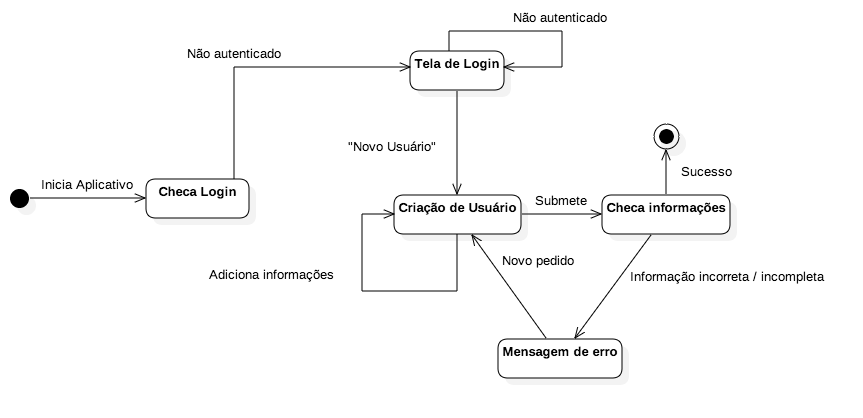
\includegraphics[scale=0.5]{state_charts/criausuario.png}
  \captionsetup{labelformat=empty}
  \caption{Figura 3.1.1: \emph{Statechart} da Criação de Usuário}
\end{figure}

\begin{figure}[h!]
  \centering
	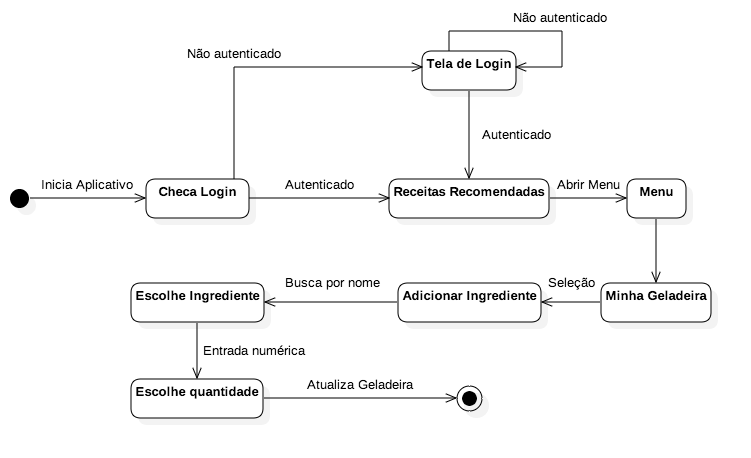
\includegraphics[scale=0.5]{state_charts/adicionaingrediente.png}
  \captionsetup{labelformat=empty}
  \caption{Figura 3.1.2: \emph{Statechart} da Adição à Geladeira}
\end{figure}

\begin{figure}[h!]
	\centering{
	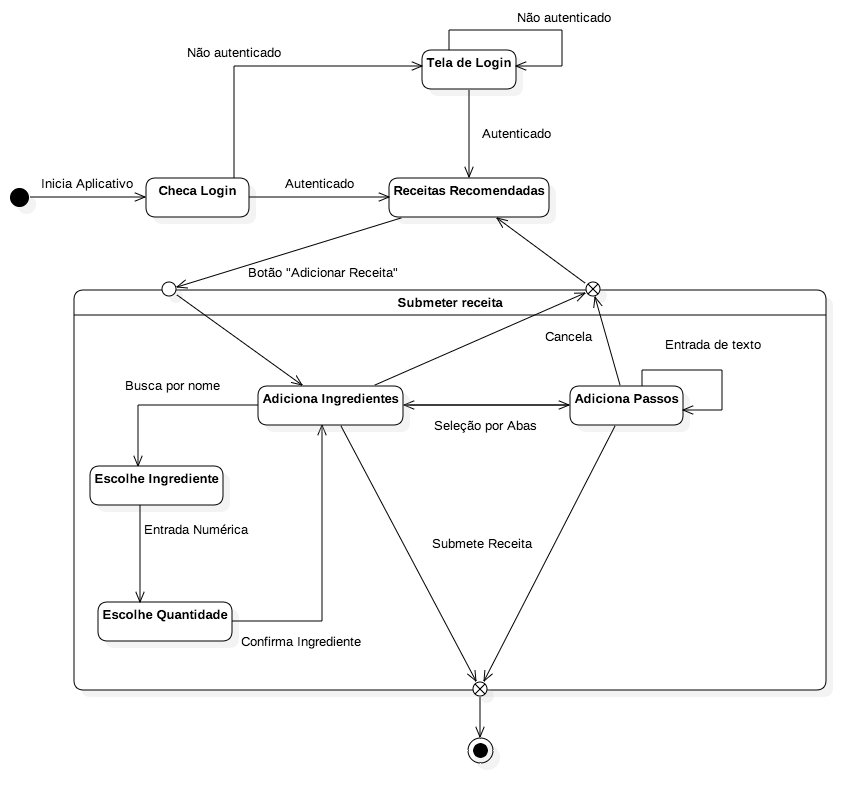
\includegraphics[scale=0.5]{state_charts/adicionareceita.png}
  \captionsetup{labelformat=empty}
  \caption{Figura 3.1.3: \emph{Statechart} da Criação de Receita}
	}
\end{figure}

\begin{figure}[h!]
	\centering
	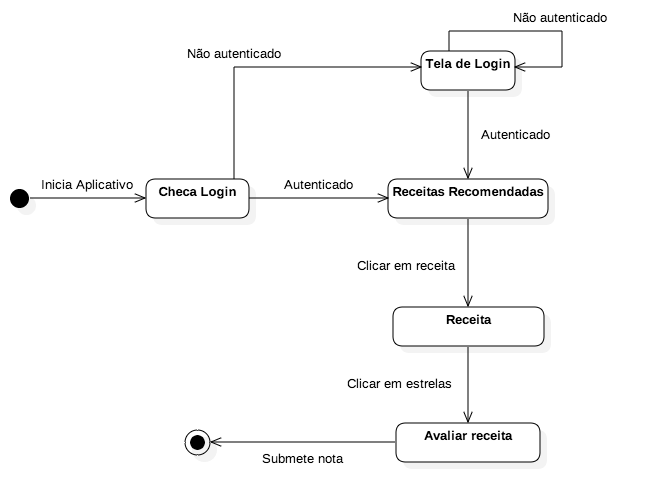
\includegraphics[scale=0.5]{state_charts/avaliareceita.png}
  \captionsetup{labelformat=empty}
  \caption{Figura 3.1.4: \emph{Statechart} da Avaliação de Receita}
\end{figure}


\end{document}
